\section{Results}
The result is a working, reliable, performant back-end, with interpreter, validator and embedded debugger.

To prove it works, three test programs were written.
All are correctly generated, all run in the interpreter, and all can be debugged.

\subsection{Test programs}
Unfortunately, since the front-end was incomplete, it is not possible to compile source files.
It \textit{is} however possible to write the front-end interface by hand.

\subsubsection{Data test}
The first test was developed to test the Data declarations.
It is equivalent to the following mc code.

\begin{MC}
Data int -> "::" -> List -> List
Data "nil" -> List

---------
main -> 0
\end{MC}

\subsubsection{List length test}
The list length program defined a list datastructure and a program to compute its length.
This was used since it uses each basic instruction at least once, as well as matching.
It is equivalent to the following MC code:

\begin{MC}
Data int -> "::" -> List -> List
Data "nil" -> List

Func "length" -> List -> int

---------------
length nil -> 0

lengtht xs -> res
---------------------
length x::xs -> res+1

--------------------------------
main -> length (1::2::3::4::nil)
\end{MC}

Which when executed prints the following on screen.

\begin{lstlisting}
4
\end{lstlisting}

This program can also be debugged with the embedded debugger.

\subsubsection{XNA test}
The second test program was to test the .Net functionality.
It consists of a simple program that modifies XNA datastructures, specifically the \verb|Vector2|.

\begin{MC}
20.0 -> x1
10.0 -> y1
Microsoft.Xna.Framework.Vector2 x1 y1 -> a
20.0 -> x2
10.0 -> y2
Microsoft.Xna.Framework.Vector2 x2 y2 -> b
Microsoft.Xna.Framework.Vector2.+ a b -> c
Microsoft.Xna.Framework.Vector2.Normalize c
y2 -> v.x 
v.x -> ret
-------------------------------------------
run -> ret
\end{MC}

Which returns \verb|20|.
This is especially intresting to debug, because we can see the values change.

\fbox{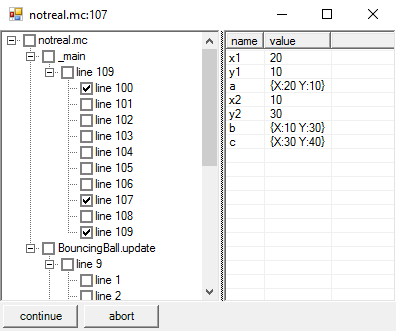
\includegraphics[width=\columnwidth-7pt]{debugger}}

